\begin{figure}[tbp]
\centering
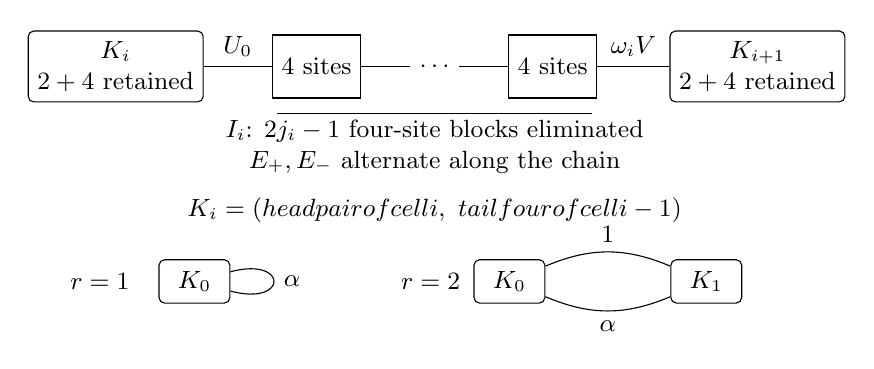
\begin{tikzpicture}[x=1cm,y=1cm,font=\small,
 core/.style={draw,rounded corners=2pt,minimum width=1.55cm,minimum height=.9cm,align=center},
 block/.style={draw,minimum width=1cm,minimum height=.8cm,align=center}]
\node[core] (kl) at (0,0) {$K_i$\\$2+4$ retained};
\node[block] (a) at (2.55,0) {$4$ sites};
\node (dots) at (4.05,0) {$\cdots$};
\node[block] (b) at (5.55,0) {$4$ sites};
\node[core] (kr) at (8.15,0) {$K_{i+1}$\\$2+4$ retained};
\draw (kl)--node[above] {$U_0$}(a);
\draw (a)--(dots); \draw (dots)--(b);
\draw (b)--node[above] {$\omega_i V$}(kr);
\draw (2.05,-.6)--(6.05,-.6);
\node[align=center] at (4.05,-1.02)
 {$I_i$: $2j_i-1$ four-site blocks eliminated\\$E_+,E_-$ alternate along the chain};
\node[align=center] at (4.05,-1.83)
 {$K_i=(\text{head pair of cell }i,\ \text{tail four of cell }i-1)$};
\node at (-.2,-2.73) {$r=1$};
\node[core,minimum width=.9cm,minimum height=.55cm] (one) at (1,-2.73) {$K_0$};
\draw (one) edge[loop right,looseness=8] node[right] {$\alpha$} (one);
\node at (4,-2.73) {$r=2$};
\node[core,minimum width=.9cm,minimum height=.55cm] (twoa) at (5,-2.73) {$K_0$};
\node[core,minimum width=.9cm,minimum height=.55cm] (twob) at (7.5,-2.73) {$K_1$};
\draw (twoa) to[bend left=23] node[above] {$1$} (twob);
\draw (twoa) to[bend right=23] node[below] {$\alpha$} (twob);
\end{tikzpicture}
\caption{Block couplings in $cI-A^2$, rather than individual graph edges.
The upper panel shows one interior chain when $j_i\ge2$; for $j_i=1$
it consists of one four-site block. The right coupling meets only the
tail-four slot of $K_{i+1}$. Eliminating all chains gives a cyclic matrix
on the $K_i$, with $\omega_i=1$ except $\omega_{r-1}=\alpha$.
The lower panels show the endpoint incidences when the cycle is a loop or
a pair of parallel chains: both contributions are added, and every core
has two incidences.}
\label{fig:boundary}
\end{figure}
